
\subsection{Resumen de objetivos}


\normalfont

El trabajo práctico consiste en el análisis del circuito de una fuente de alimentación lineal realimentada. El análisis es por cálculo y por simulación con \textbf{SPICE} (\textbf{LTSPICE} específicamente en nuestro caso), de donde se pretende obtener una caracterización de la fuente de alimentación. Un detalle a mencionar es que los datos de las simulaciones se exportaron a archivos de texto con los datos crudos de las señales y se procesaron y graficaron en \textbf{MATLAB}, principalmente para mayor detalle y precisión en los gráficos, pero también nos simplificó los cálculos.


\subsection{Desarrollo}

Se hace un análisis cualitativo de la fuente para luego pasar a analizar las diferentes secciones del circuito, remitiendo a apartados donde sea necesario, para explicar conceptualmente algún subcircuito, luego haciendo una análisis de pequeña señal a frecuencias bajas y medias, para finalmente usando esta información, responder las preguntas propuestas en las consignas del trabajo práctico.
En la figura~\figref{fig:fig_complete_circuit_secions} se muestra el circuito completo usado para la simulación donde se puede ver las subsecciones que se analizarán, en el mismo también se muestran los puntos de reposo obtenidos para una condición particular de carga.

\clearpage


\begin{figure}[H] %htb
\begin{center}
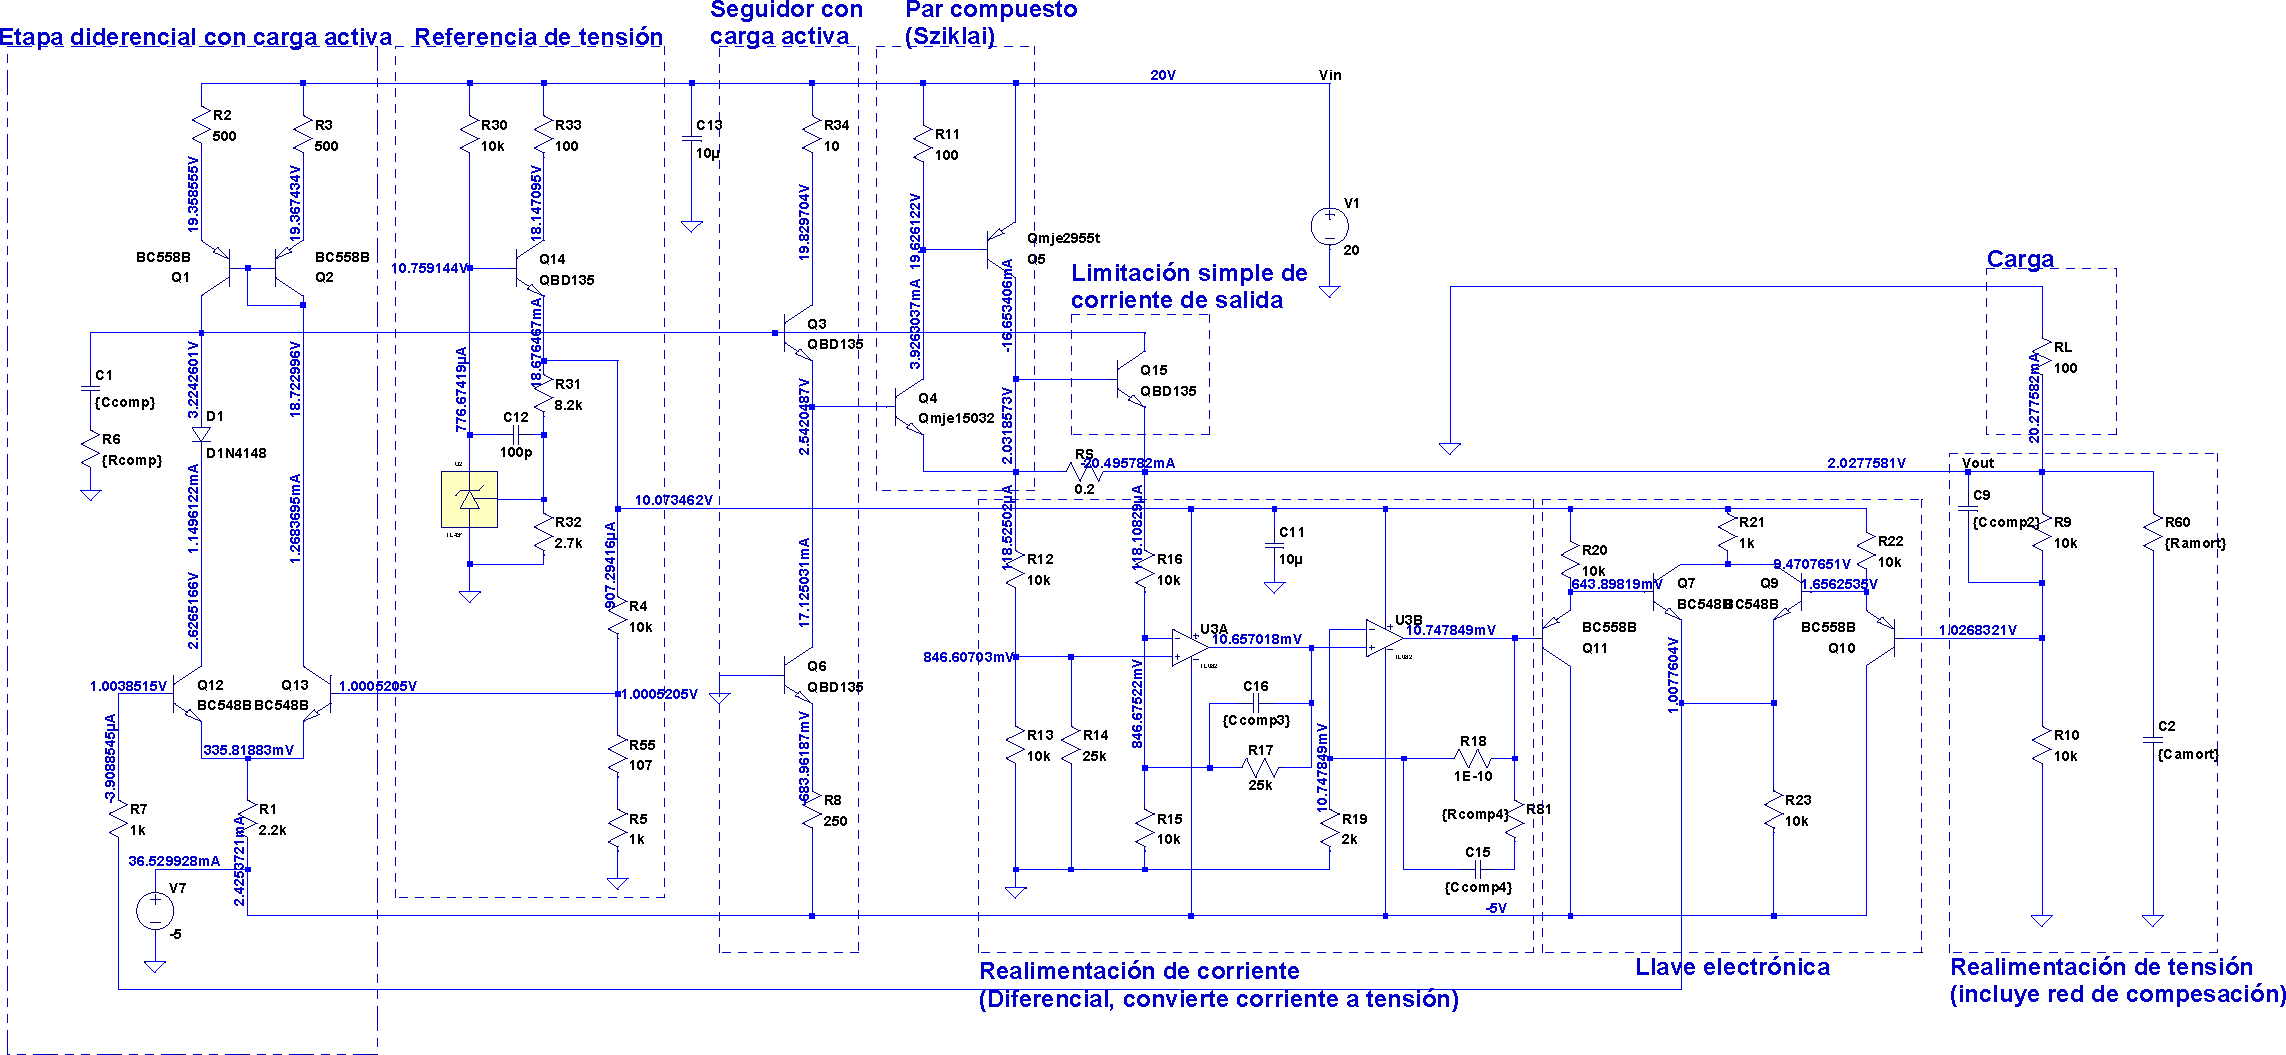
\includegraphics[width=1.2 \textwidth, angle=90]{./img/desarrollo/power_supply_subsections.png}
\caption{\label{fig:fig_complete_circuit_secions}\footnotesize{Circuito completo con las secciones indicadas.}}
\end{center}
\end{figure}
